\section{The investigation record}
\label{sec:state}

\subsection{What connects one step to the next}
\label{sec:state-transition}

A graph drawing shows where control is allowed to go, and it says nothing about what travels along
the edges. What travels is one record, and the mechanisms of the two sections that follow, routing
and dispatch, are both defined over it.

\begin{definition}[State and the state schema]
\label{def:state}
State is ``a shared data structure that represents the current snapshot of your
application''~\citep{langgraph-graph-api}. It is declared as a schema, a named set of fields with
their types, which every node receives as input and updates as output.
\end{definition}

We write one step of a run as two operations rather than one. A node reads the current state
$s_t$ together with a result $e_t$ that arrived from outside the program, and it returns a partial
update $u_t$. The runtime then merges that update into the record, key by key:
\[
  u_t \;=\; \mathrm{node}(s_t,\, e_t), \qquad
  s_{t+1} \;=\; \mathrm{merge}(s_t,\, u_t).
\]

\begin{figure}[htbp]
  \centering
  \begin{adjustbox}{width=\linewidth}% One transition: a node reads state and an external result, returns a partial update, and the
% runtime merges that update key by key. The dashed edge is the reducer's left argument, which
% comes from the current state and never from the node.
\begin{tikzpicture}[node distance=6mm and 5mm]
  \node[rnode] (s0) {state $s_t$};
  \node[mnode, right=of s0] (node) {node};
  \node[gnode, right=of node] (upd) {partial\\update $u_t$};
  \node[rnode, right=15mm of upd] (red) {reducer,\\one per key};
  \node[rnode, right=of red] (s1) {state $s_{t+1}$};
  \node[tnode, align=center, below=8mm of node] (ext) {model reply or\\tool observation $e_t$};
  \draw[flow] (s0) -- (node);
  \draw[flow] (node) -- (upd);
  \draw[flow] (upd) -- node[lab, below] {right\\argument} (red);
  \draw[flow] (red) -- (s1);
  \draw[flow] (ext) -- (node);
  \draw[back] (s0.north) to[out=35, in=145] node[lab, above] {left argument} (red.north);
\end{tikzpicture}
\end{adjustbox}
  \caption{One transition. The node proposes an update; the runtime merges it. Each key is merged
  by its own reducer, whose left argument is the value already in state and whose right argument is
  the value the node returned.}
  \label{fig:state-transition}
\end{figure}

The term $e_t$ makes explicit what the current state does not determine. A model reply is sampled
from a distribution, while a tool observation depends on a fixture that the run itself may have
modified. Neither result is determined by $s_t$ alone. This is the nondeterminism discussed in
\cref{sec:agents-properties}: \textbf{the same state can produce different successors}. A run can
therefore go wrong at this boundary even when every node behaves correctly.

A node returns only the keys it touched, because ``the Node does not need to return the whole State
schema - just an update''~\citep{langgraph-graph-api}. Our controller returns three keys out of the
loop's ten, \demoref{messages}, \demoref{model\_calls} and \demoref{usage}, and it returns a
single key, \demoref{status}, on the two paths where it stops the run before issuing a call.

The runtime, not the node, decides what merging means. It applies one reducer per updated key and
saves the result, which is why a node can be written without knowing whether its contribution will
be appended to a list or will overwrite what is there. Execution proceeds in super-steps, where ``a
super-step can be considered a single iteration over the graph nodes''~\citep{langgraph-graph-api},
and the record is consistent at each super-step boundary rather than inside a node.

\subsection{Model context, runtime state, durable state}
\label{sec:state-three}

Model context and runtime state are easy to confuse because much of their content overlaps.
The model sees only what it needs for the current call; the runtime also tracks counters and other
fields used to control execution. Saving enough of that state to resume after the process ends
makes it durable.

\begin{table}[htbp]
  \centering
  \begin{adjustbox}{width=\linewidth}\begin{tabularx}{\linewidth}{@{}L{0.19\linewidth}X@{}}
    \toprule
    \textbf{Record} & \textbf{What it holds, and who reads it} \\
    \midrule
    Model context & The instructions, the selected history, and the observations supplied to one
    model invocation. Assembled per call, read by the model. \\
    Runtime state & The record the runtime maintains between steps, including fields that enter
    no model call. Read by nodes, by routing functions, and by the limits we enforce. \\
    Durable state & State written somewhere that survives the end of the process, in a form that
    supports resuming a run rather than restarting it. \\
    \bottomrule
  \end{tabularx}\end{adjustbox}
  \caption{Three records, kept apart. Model context is derived from runtime state at each call;
  durable state is runtime state that has been written down.}
  \label{tab:state-three}
\end{table}

The counters are the clearest case of a field that stays behind. Our loop refuses a model call once
\demoref{model\_calls} reaches forty and once the last three observations came back identical, and
neither number is shown to the model. We keep them out on purpose: a limit the model can read is a
limit the model can argue with, and we want the check to be a comparison in the controller rather
than an instruction in a prompt.

Now, durability. Kill the process in the middle of a run and start it again: what does the agent
still know? For the loop as it stands, nothing. The record lives in memory, so a terminated process
takes the whole investigation with it, and in-memory state is state all the same. The framework's
answer is to compile the graph with a checkpointer, which gives ``agents short-term memory'' and
``lets LangGraph applications keep useful information beyond a single graph
run''~\citep{langgraph-persistence}.

Here, \emph{durable} means only that the record can be read back after the process that wrote it is
gone. It does not mean that resuming is free of consequences. Checkpoints are saved at super-step
boundaries and not inside a node, so a run that resumes re-enters the interrupted node from its
first line and repeats whatever that node had already done, including the calls it had already
paid for. Persistence and recovery are taken up properly in the later units; what the record has to
carry for this lecture is the run, not the restart.

\subsection{The record is factored}
\label{sec:state-factored}

How much structure a state record has is a design decision with consequences, and the ways of
representing a state lie on an axis of increasing expressive power: atomic, factored, and
structured \citep[\S2.4.7]{russell2020aima}. In an atomic representation each state is
indivisible, a black box whose only property is being the same as or different from another. A
factored representation splits each state into a fixed set of variables, each with a value. A
structured representation describes objects, each with attributes of its own and relationships to
other objects.

\begin{figure}[htbp]
  \centering
  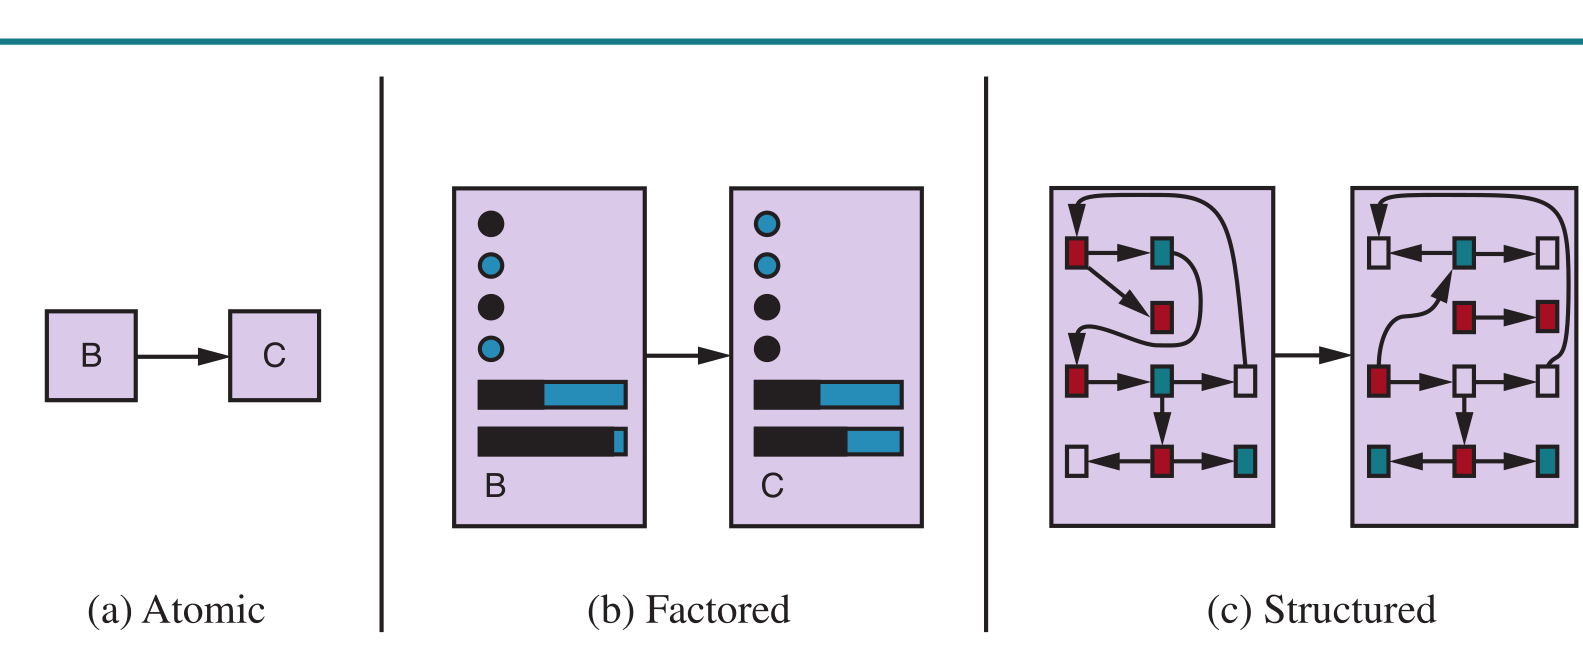
\includegraphics[width=\linewidth]{figures/aima-fig2-16.png}
  \caption{Three ways to represent states and the transitions between them. Figure~2.16 of
  \citet{russell2020aima}, reproduced from the Global Edition (\copyright~Pearson Education
  Limited 2022).}
  \label{fig:state-fig216}
\end{figure}

\msa{} uses all three, in different places.

\bi

\item \textbf{Atomic.} The outcome of the run. Accepted or stopped is a label with no internal
structure, and two runs that end in the same label are indistinguishable at that level. The number
a benchmark reports is a count of such labels.

\item \textbf{Factored.} The record itself. The alert, the observations, the candidate patch, the
counters and the status are named fields with values, and two states can agree on some and differ
on others.

\item \textbf{Structured.} The patch and the rejection. A patch is a set of hunks, each over a file
and a range of lines; a rejected submission names the check that failed, the file, and the line.

\ei

Keeping the record factored is what buys us the machinery of the rest of Part~B: one reducer per
named field (\cref{sec:state-reducers}), routing predicates that read a field rather than parse a
sentence (\cref{sec:control}), and limits that are comparisons on a counter. Structure is confined
to the two values where the model has to defend its work, and \textbf{the expressive representation is
the exception rather than the default}, because reasoning over structure is harder for us and for
the model both \citep[\S2.4.7]{russell2020aima}.

\Cref{tab:state-fields} is the schema as \demoref{state.py} declares it. Its fields have three lifetimes: i) identity, set once, ii)
run-local, carried across the whole run, and iii) attempt-local, cleared when the reflection step
starts a new attempt.

\begin{table*}[tbp]
  \centering
  \begin{adjustbox}{width=\linewidth}\begin{tabularx}{\linewidth}{@{}L{0.20\linewidth}L{0.155\linewidth}L{0.155\linewidth}X@{}}
    \toprule
    \textbf{Field} & \textbf{Lifetime} & \textbf{Reducer} & \textbf{What it holds} \\
    \midrule
    \demoref{alert}, \demoref{repo}, \demoref{commit}, \demoref{workspace}
      & identity & none & The scanner alert under investigation, the fixture, the
        pinned commit, and the copy of the tree this run may touch. \\
    \demoref{messages} & run-local & append & The conversation, in provider form. \\
    \demoref{observations} & attempt-local & append & One record per dispatched tool call, whether
      it succeeded or was refused. \\
    \demoref{candidate\_patch} & attempt-local & replace & The patch currently proposed. \\
    \demoref{plan} & attempt-local & replace & The subgoals and their status, written by the
      planner. \\
    \demoref{validation} & attempt-local & replace & The latest acceptance decision and its
      reasons. \\
    \demoref{reflections} & run-local & append & Guidance retained from attempts that were
      rejected. \\
    \demoref{attempt} & run-local & explicit & Which attempt is running, under the runtime's
      control. \\
    \demoref{model\_calls}, \demoref{usage} & run-local & accumulate & Calls issued and tokens
      spent, kept across attempt resets. \\
    \demoref{status} & run-local & replace & Running, or the terminal status that ended the run. \\
    \bottomrule
  \end{tabularx}\end{adjustbox}
  \caption{The state schema of \demoref{state.py}. The loop populates the identity fields,
  \demoref{messages}, \demoref{observations}, \demoref{candidate\_patch}, the counters and
  \demoref{status}; each later version adds the field its new node fills, so a version's diff shows
  one change rather than a field that was always waiting.}
  \label{tab:state-fields}
\end{table*}

Nothing in that declaration checks anything. A \demoref{TypedDict} is a description for a type
checker, not a gate: its types cannot be used in \demoref{isinstance} tests, and an instance
``returns an ordinary dictionary object at runtime''~\citep{pep589}. A model reply that puts a
string where the schema declares an integer produces a state that type-checks in the editor and is
wrong at run time, and the check that catches it is the argument validation of
\cref{sec:boundary}, which we wrote.

\subsection{Reducers, and what a later step is allowed to see}
\label{sec:state-reducers}

A reducer is a small function with a large consequence: it decides whether a field accumulates a
history or keeps only its latest value, and therefore what evidence is available to every step that
comes after.

\begin{definition}[Reducer]
\label{def:reducer}
``Each key in the State has its own independent reducer function''~\citep{langgraph-graph-api}.
Every reducer is a binary function of two positional arguments, the value already stored in state
for that key and the update returned by a node, and where none is specified the default applies:
it ``ignores the left argument and replaces the state value with the right
argument''~\citep{langgraph-graph-api}.
\end{definition}

We use three, and each one answers a question about visibility rather than about storage.

\bi

\item \textbf{Append.} \demoref{observations} is annotated with \demoref{operator.add} and
\demoref{messages} with \demoref{add\_messages}, so every tool result of the current attempt stays
readable. The controller's stall check needs exactly this: it compares the last three observations
and stops the run when they are identical, which is a question no replaced field could answer.

\item \textbf{Replace.} \demoref{candidate\_patch}, \demoref{plan}, \demoref{validation} and
\demoref{status} take the default. Each names what is true now, and a superseded plan is not
evidence of anything except that the run changed its mind.

\item \textbf{Accumulate.} \demoref{usage} is merged by \demoref{add\_usage}, which sums four token
counters and produces no total. Each node reports only the cost of its own call, so no node ever
holds the running total and no node can overwrite it. The four counters stay apart because they
are not interchangeable: a cache read costs a fraction of fresh input, and a single number cannot
answer whether cache reads rose while fresh input fell.

\ei

The reset between attempts is where these choices are felt. When the validator rejects a candidate
and the reflection step writes guidance for the next try, the new attempt has to begin with the
attempt-local fields cleared and the run-local ones intact. Returning an empty list for
\demoref{observations} does not do it: \textbf{an append reducer given an empty update leaves every
earlier observation exactly where it was}, so the next attempt would inherit the reasoning it was
supposed to be freed from. Clearing a field with an append reducer takes an explicit assignment
under the runtime's control, and the runtime records it in the trace as a state change. Identity,
reflections, the counters and the usage ledger survive the reset by design, because an attempt
limit enforced on a counter that resets with the attempt is not a limit at all.

\subsection{The demo: one tool result becoming state}
\label{sec:state-demo}

Four events into \demoref{runs/v1-bc284c6b.jsonl}, the model has asked to read the file the alert
names, and the dispatcher has returned 1,665 characters of source. \Cref{fig:state-views} shows
the record before the merge, the update the \demoref{tools} node returns, and the model input
assembled from the result.

\begin{figure}[htbp]
\begin{lstlisting}[basicstyle=\ttfamily\scriptsize, columns=fixed,
literate={"}{{\textquotedbl}}1]
# 1. state before the merge (the keys this transition touches)
{"messages": [system, user, ai(tool_call read_file)], "observations": [],
 "model_calls": 1, "usage": {"input": 914, "output": 49, ...}, "status": "running"}

# 2. the update the tools node returns, and the merged result
return {"observations": [{"tool": "read_file",
                          "args": {"path": "testcode/BenchmarkTest00283.py"},
                          "ok": True, "result": "<1665 chars of source>"}],
        "messages": [ToolMessage(content=..., tool_call_id=...)]}
# merged: observations grows by one (operator.add), messages grows by one
# (add_messages), and every other key is untouched because it was not returned

# 3. the next model input, assembled from state["messages"] alone
[system, user, ai(tool_call read_file), tool(result)]
\end{lstlisting}
  \caption{One tool result entering the record, from \demoref{runs/v1-bc284c6b.jsonl}, steps 3
  and 4. The node names two keys; the runtime merges each one by its own reducer.}
  \label{fig:state-views}
\end{figure}

Three things in that transition are worth holding on to. The node returned two keys and the
loop's record has ten, so the counters advanced only where a node said so. The observation the runtime
stored is richer than the message the model receives, because it keeps the arguments and the
success flag alongside the text, and routing and accounting read those fields rather than the
prose. And the model input for the next call is built from \demoref{messages} alone:
\demoref{model\_calls} stood at one throughout and was never shown, which is precisely how a
budget stays a runtime control.

The trace is a fourth record, and it is the one that outlives the process. Every transition worth
auditing is written to it as an event, \demoref{tool\_request} and \demoref{tool\_result} from the
dispatcher, \demoref{model\_call} from the controller, \demoref{routing} from the conditional
edges, \demoref{state\_change} from an attempt reset, and \demoref{terminal} once, at the end.
State answers what the run knows now; the trace answers what the run did, and
\cref{sec:control} rests on the second.

\subsection{Exercises}

\begin{enumerate}
\item Take the schema of \cref{tab:state-fields} and mark, for each field, whether the model ever
  sees its value. For every field you mark ``no'', say which decision in the runtime reads it.
\item \demoref{add\_usage} sums four counters and produces no total. Write the one question about a
  run that a single total makes unanswerable, and name the pair of counters whose movement answers
  it.
\item A colleague clears \demoref{observations} between attempts by returning an empty list for
  that key from the reflection node. Say what the record contains after the update is merged, and
  give the smallest change that produces the intended reset.
\item Our controller refuses a model call once forty calls have been issued. Suppose instead the
  limit were stated in the system prompt and the counter were removed from state. Name one run in
  which the two designs give different outcomes, and say which record you would inspect to tell
  them apart.
\end{enumerate}

\subsection{Reading}

\citet{langgraph-graph-api}, the sections on state, schemas, reducers and
super-steps, which are the implementation reference for everything in this section. \S2.4.7 of
\citet{russell2020aima} supplies the atomic, factored and structured distinction and
Figure~2.16.

For reference while writing HW1: \citet{pep589} on what a \demoref{TypedDict} does and does not
check at run time, and \citet{langgraph-persistence} on checkpointers, threads and stores, which is
the machinery behind the durability row of \cref{tab:state-three}.

\paragraph{Looking ahead.} The record is now the thing every later mechanism reads. The next
section takes the code that reads it to choose the next node, and choosing to stop is one of those
choices. We work through conditional edges, the two back edges that return a run to the planner,
and three endings that a trace can establish: a run that completed, a run that declared a stop, and
a run whose trace records no ending at all.
